\newpage
\section{Изменения в компиляторе}
В рамках данной главы будут описаны изменения в компиляторе, направленные на решение проблем,
найденных в разделе \ref{section:benchmarks}.

\subsection{Архитектура компилятора}
Большинство современных компиляторов, включая Kotlin, реализуют архитектурный шаблон, описанный
в \cite{Muchnick}.

Его суть состоит в разделении всего кода на следующие компоненты, каждая из которых должна зависеть
только от предыдущих:
\begin{enumerate}
    \item \textit{Лексический анализатор} --- принимает на вход содержимое программы в виде строки
    символов, и выдает поток семантически значимых фрагментов, т.н. <<токенов>>.

    \item \textit{Синтаксический анализатор} --- реализует один из алгоритмов синтаксического
    анализа и строит из потока <<токенов>> абстрактное синтаксическое дерево.

    \item \textit{Семантический анализатор}, получая абстрактное синтаксическое дерево, производит
    вывод типов выражений, если это необходимо, и проверяет корректность программы с точки зрения
    спецификации языка и его системы типов.

    \item \textit{Генератор кода} --- подсистема, генерирующая по размеченному синтаксическому
    дерево код для целевой архитектуры, в случае Kotlin --- class-файлы виртуальной машины Java.
\end{enumerate}

Для данной работы наибольший интерес, очевидно, представляет именно генератор кода.
Его часть, отвечающая за генерацию байт-кода методов представлена в виде класса, реализующего
шаблон проектирования <<Посетитель>>\cite{Gamma}, каждый ``visit''-метод которого отвечает за
генерацию отдельного вида узлов синтаксического дерева и чаще всего выполняет контракт,
гарантирующий, что результат аргумента-выражения окажется на вершине стека.

\subsection{Безопасный вызов и elvis-оператор}
\label{section:elvis:op}
%\begin{verbatim}
                %aload_1 // Загрузка `obj` на стек
                %dup
                %ifnull l1
                %getfield x
                %invokestatic  java/lang/Integer.valueOf() // Боксинг
                %goto          l3
                %l1: pop
                %aconst_null
                %// начало кода elvis-оператора
                %l2: dup
                %ifnull l3
                %invokevirtual java/lang/Number.intValue() // Распаковка
                %goto          l4
                %l3: pop
                %iconst_1
                %l4: ...
%\end{verbatim}

В разделе \ref{section:elvis:bm} были описаны произведенные измерения, демонстрирующие низкую
производительность байт-кода для сочетания безопасного вызова и elvis-оператора.

Ниже произведен более подробный анализ байт-кода бенчмарков и описаны решения для оптимизации.

\begin{figure}
\begin{center}
    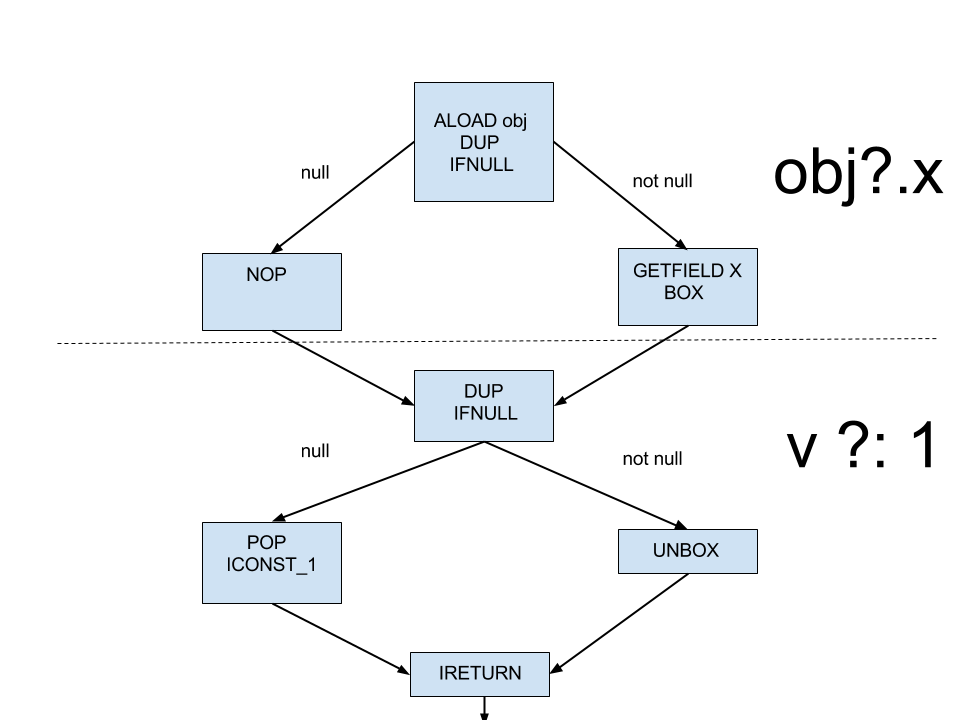
\includegraphics[scale=0.4]{../resources/safecall_elvis.png}
\end{center}
\caption{Блок-схема байт-кода для выражения ``return (obj?.x ?: 1)''}
\label{sc:elvis}
\end{figure}

Примерная блок-схема байт-кода бенчмарка изображена на рисунке \ref{sc:elvis}.
Часть, расположенная выше пунктирной линии описывает генерацию безопасного вызова:
\begin{itemize}
    \item На стек загружается переменная ``obj'', ее значение копируется с помощью инструкции
    ``DUP'', и копия проверяется на равенство ``null''.
    \item В случае если ``obj'' является нулевой ссылкой, то лежащее на вершине стека значение
    тоже нулевая ссылка.
    Иначе на стеке лежит объект ``obj'', у которого берется значение в поле ``x'' и упаковывается.
\end{itemize}

Таким образом обеспечивается контракт безопасного вызова, и на вершине стека находится либо нулевая
ссылка, либо упакованное значение поля.

Боксинг в данном случае необходим, так как ситуация, когда при одном потоке исполнения в ячейке
стека значение примитивного типа, а при другом --- ссылка, запрещена спецификацией виртуальной
машины\cite{JVMSpec}.

Вторая часть блок-схемы иллюстрирует байт-код для elvis-оператора:
\begin{itemize}
    \item Значение, лежащее на вершине стека, копируется и проверяется на равенство нулевой ссылке.
    \item В случае, если оно является нулевой ссылкой, то его копия снимается со стека и
    загружается значение по умолчанию --- целочисленная константа <<1>>.

    Иначе не стеке лежит объект класса ``java.lang.Integer'', из которого и получается значение
    с помощью вызова метода ``intValue'', на блок-схеме этот вызов отмечен для простоты, как
    ``UNBOX''.
\end{itemize}

Понятно, что байт-код этих операторов по отдельности наиболее очевидным образом выражает
их семантику, и выразить их еще проще в рамках спецификации JVM, пожалуй, не представляется
возможным.
Однако их сочетание ни в коей мере оптимальным не кажется.

\begin{figure}
\begin{center}
    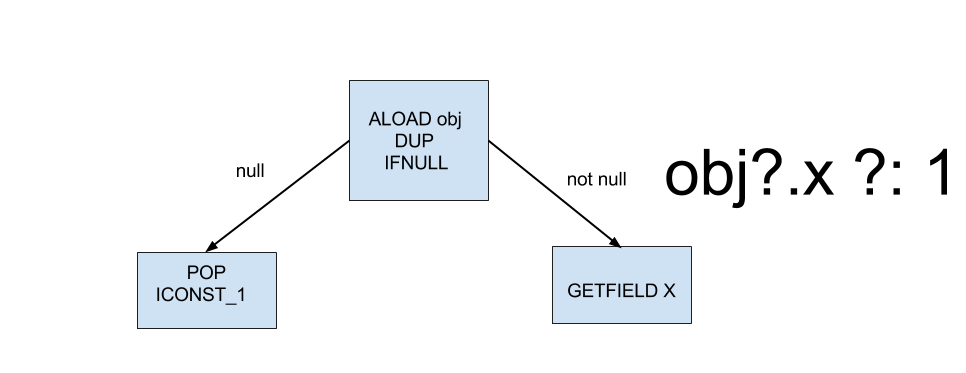
\includegraphics[scale=0.4]{../resources/safecall_elvis_optim.png}
\end{center}
\caption{Блок-схема байт-кода для выражения ``return (obj?.x ?: 1)'' (оптимальный вариант)}
\label{sc:elvisOpt}
\end{figure}

Наиболее кратким вариантом трансляции кажется изображенный на рисунке \ref{sc:elvisOpt}:
\begin{itemize}
    \item Переменная ``obj'' загружется на стек, создается ее копия, и сравнивается с нулевой
    ссылкой.
    \item Если значение является нулевой ссылкой, то его копия снимается со стека, и загружается
    значение по умолчанию.
    Иначе на вершине стека хранится объект, у которого берется значение поля ``x''.
\end{itemize}

При такой генерации отсутствуют операции боксинга, что, как выяснилось в рамках измерений,
хуже всего влияет на производительность вышеописанного байт-кода.

\paragraph{Решение}
В связи с условной оптимальностью байт-кода для операторов по отдельности, наиболее разумным
решением кажется специализация кодогенерации для выражений вида: $x_1?.x_2?...?.x_k\ ?: default$
в соответствие с идеей, проилюстрированной на рис. \ref{sc:elvisOpt}.

Упрощенно суть изменений можно выразить в виде следующего псевдокода:
\begin{lstlisting}[frame=single]
    function genElvis(v1: Expr, v2: Expr) {
        if (v1 is SafeCallChain) {
            // v1 ~ x1?.x2?...?.xk
            genSafeCallChain(v1, defaultLabel);
        } else {
            gen(v1);
        }

        DUP();
        IFNULL(defaultLabel);

        // ifNullLabel starts here
        gen(v2);
    }

    function genSafeCallChain(v: safeCallChain, ifNullLabel: Label) {
        for (element in v) {
            gen(v);
            DUP();
            IFNULL(ifNullLabel);
        }
    }
\end{lstlisting}

По сути логика генерации осталась прежней за исключением изменения генерации безопасных вызовов:
при проверке аргумента на равенство нулевой ссылке, сразу происходит переход к инструкции,
с которой начинается генерация значения по умолчанию.

Аналогичная оптимизация была произведена и для цепочки безопасных вызовов вне elvis-оператора,
в таком случае код можно генерировать по аналогии с выражением ``x1?.x2?..?.xk ?: null''.

В совокупности с изменениями, описанными в следующем разделе, это решение способствовало улучшению
производительности байт-кода, как микро-бенчмарков из раздела \ref{section:elvis:bm}, так и кода
АВЛ-дерева из раздела \ref{section:avl:bm}.
Результаты измерений в таблицах \ref{bm:elvis:o} и \ref{bm:stars:o}.

\begin{table}[h]
\begin{center}
\begin{tabular}{|c|c|c|c|c|} \hline
$p$ & Эталон (мкс) & До оптимизаций (мкс) & После оптимизаций (мкс) & Ускорение \\ \hline
0.1 & 4.693 $\pm$ 0.036 & 9.131 $\pm$ 0.126 & 4.619 $\pm$ 0.039 & 1.977\\ \hline
0.5 & 7.103 $\pm$ 0.078 & 7.138 $\pm$ 0.263 & 7.105 $\pm$ 0.039 & 1.005\\ \hline
0.9 & 4.561 $\pm$ 0.043 & 4.738 $\pm$ 0.047 & 4.523 $\pm$ 0.064 & 1.048\\ \hline
\end{tabular}
\caption{Результаты бенчмарка "Безопасный вызов и elvis" после оптимизаций \newline (p --- вероятность нулевой ссылки)}
\label{bm:elvis:o}
\end{center}
\end{table}

\begin{table}[h]
\begin{center}
\begin{tabular}{|c|c|c|c|c|} \hline
Размер & Java & Kotlin & После оптимизаций & Ускорение \\ \hline
100 & 19.412 $\pm$ 0.266 мкс & 30.687 $\pm$ 1.66 мкс & 21.837 $\pm$ 0.309 мкс & 1.405\\ \hline
1000 & 300.055 $\pm$ 2.397 мкс & 476.807 $\pm$ 4.243 мкс & 335.531 $\pm$ 11.768 мкс & 1.421\\ \hline
100000 & 78.686 $\pm$ 3.14 мс & 132.768 $\pm$ 3.938 мс & 79.394 $\pm$ 1.896 мс & 1.672\\ \hline
\end{tabular}
\caption{Результаты бенчмарка <<АВЛ-дерево>> после оптимизаций}
\label{bm:stars:o}
\end{center}
\end{table}

\subsection{Оператор when для константных выражений}
\label{section:when:opt}
Измерения, результаты которых изложены в разделе \ref{section:when:bm}, показали, что использование
байт-код инструкций ``tableswitch'' и ``lookupswitch'' для оператора ``when'' с константными
выражениями может значительно улучшить производительность соответствующего участка байт-кода.

Эти инструкции объединяет общая семантика:
\begin{itemize}
    \item Они параметризуются отображением из набора целых чисел в указатели на другие инструкции
    метода.
    \item При исполнении инструкции интерпретатор снимает с вершины стека число и совершает
    соответствующий переход.
\end{itemize}

Различия заключаются в том, что
\begin{itemize}
    \item \textit{tableswitch} параметризуется интервалом $[high..low]$.
    Для каждого целочисленного значения из этого интервала должна быть задана метка перехода,
    а кроме этого указатель на инструкцию по умолчанию.

    Таким образом размер этой инструкции линейно зависит от ширины интервала.
    \item \textit{lookupswitch} параметризуется отсортированным набором пар значений и меток
    перехода.

    Размер такой инструкции зависит линейно от числа значений.
\end{itemize}

Несмотря на то, что в спецификации не указана трудоемкость выполнения этих инструкций, из формата
их описания понятно, что ``tableswitch'' может быть исполнен за $O(1)$ прямым вычислением индекса
следующей инструкции, а ``lookupswitch'' может быть реализован на основе бинарного поиска и
работать за $O(log\ n)$.

\paragraph{Выбор инструкции}
Сама по себе задача генерации специальных инструкций для случая, когда все выражения
для сопоставления в ``when'' --- константы, не представляется алгоритмически сложной, с учетом
наличия в компиляторе подсистемы для вычисления констант времени компиляции.

Однако существует некоторое количество тонкостей, о которых следует упомянуть в рамках данного
раздела.

Например при реализации неизбежно возникает проблема выбора между двумя инструкциями,
являющаяся по сути задачей многокритериального анализа:
\begin{itemize}
    \item ``tableswitch'' вероятно более производительна, но ее размер в байт-коде линейно
    пропорционален ширине интервала.
    \item ``lookupswitch'' более компактна, ее размер в байт-коде пропорционален числу меток.
\end{itemize}

В результате было принято решение воспользоваться эвристическим алгоритмом, который используется
для выбора инструкции в компиляторе Java из набора OpenJDK\fu{https://github.com/openjdk-mirror/jdk7u-langtools/blob/9f03d0c131f6343fee00f5dc5485c047e5cd2033/src/share/classes/com/sun/tools/javac/jvm/Gen.java\#L1159}:
\begin{itemize}
    \item Для каждого из вариантов вычисляется его условная стоимость как сумма стоимостей
    по памяти и производительности в виде числа сравнений --- $spaceCost + 3 * timeCost$

    \item Для ``tableswitch'' его стоимость по памяти полагается равной числу занимаемых машинных
    слов, т.е. $spaceCost = 4 + (high - low)$.

    Его трудоемкость оценивается значением $timeCost = 3$: два сравнения, необходимые для проверки,
    что данное число помещается в интервал $high..low$, и одно действие для безусловного прыжка.

    \item Для ``lookupswitch'': $spaceCost = 3 + 2 * n, timeCost = n$, где $n$ --- число меток.

    \item Вычисленные условные стоимости сравниваются и выбирается вариант с наименьшим
    результатом.
\end{itemize}

\paragraph{Оператор when для строк}
Для эффективного использования switch-инструкций, которые могут работать только с целочисленными
аргументами, при сравнении строк, используется хеш-функция, определенная в классе
``java.lang.String''.

Разумеется из равенства значений хеш-функций нельзя делать выводы о равенстве строк,
поэтому в каждой метке switch-инструкции необходимо произвести соответствующие проверки.

Также следует обработать редкий случай, когда коллизии возникают между различными строками
из набора выражений для сопоставления.

Получаемый при генерации байт-код мог бы быть получен при компиляции следующего кода,
если бы в Java был реализован оператор ``goto''.
\begin{pyglist}[language=java]
String tmp0 = x;
switch(tmp0.hashCode()) {
    case 101584: if (tmp0.equals("foo")) { goto l1; }
    case 97299: if (tmp0.equals("bar")) { goto l2; }
}
l1: ...
l2: ...
\end{pyglist}

Любопытной деталью, является тот факт, что в компиляторе Java оператор ``switch'' для строк еще
до фазы генерации кода трансформируется в ``switch'' для целочисленных значений примерно такого же
вида, как изображенный выше код.
Однако ввиду отсутствия в языке конструкции ``goto'' его поведение эмулируется сохранением
во временную переменную номера совпавшей строки и дополнительным ``switch'' от этой переменной.

А так как изменения в компиляторе Kotlin производились внутри фазы кодогенерации, автору удалось
избавитсься от этой избыточности, и таким образом получить версию примерно на 10\% эффективней
версии Java (см. таблицу \ref{bm:switch:opt}).

\paragraph{Оператор when для enum-классов}
Для использования ``switch''-инструкций при генерации when для enum-классов использовался метод
``ordinal()`` определенный для каждой enum-константы, и возвращающий ее порядковый номер.

Однако компилятор Java выполняет дополнительную микрооптимизацию:
\begin{itemize}
    \item Для каждого класса, в котором вызывается ``switch'' от enum-класса, создается
    синтетический вложенный класс со статическими полями-массивами --- по одному на каждый такой
    ``switch''.
    \item Каждый массив имеет размер равный числу enum-констант в конкретном классе, и имеет смысл
    отображения порядковых номеров констант, используемых в метках, в последовательные номера
    от единицы.
    \item И вместо ``switch'' по непосредственному значению ``ordinal()`` генерируется ``switch''
    по элементу в соотвествующем массиве с индексом ``ordinal()''
\end{itemize}

Эта оптимизация, как следует из комментария к исходному коду, направлена на то, чтобы гарантировать
эффективное использование ``tableswitch'' при генерации оператора ``switch'' для enum-классов.

Реализация оптимизации ``when'' в Kotlin была сделана аналогично, в результате чего получаемый
байт-код можно проиллюстрировать следующим кодом на Java:
\begin{pyglist}[language=java]
    switch(CurrentClass$Mappings.$Mapping0[x.ordinal()]) {
        case 0: // ...
        case 1: // ...
        ...
    }
\end{pyglist}

\paragraph{Измерения после оптимизаций}
После внедрения описанных выше оптимизаций результаты бенчмарков, описанных
в разделе \ref{section:when:bm}, стали аналогичным результатам эталонных версий, написанных
на Java, кроме бенчмарка со строками, который стал производительней <<эталонного>> варианта на 10\%.

\begin{table}[h]
\begin{center}
\begin{tabular}{|c|c|c|c|c|} \hline
Разреженность & Java (мкс) & Kotlin (мкс) & После оптимизаций (мкс) & Ускорение \\ \hline
1..20 & 4.281 $\pm$ 0.018 & 7.8 $\pm$ 0.131 & 4.284 $\pm$ 0.029 & 1.821\\ \hline
1..20, 100500 & 5.554 $\pm$ 0.077 & 7.524 $\pm$ 0.065 & 5.55 $\pm$ 0.068 & 1.356\\ \hline
\end{tabular}
\caption{Сравнение производительности операторов switch/when для целочисленных констант после оптимизаций}
\end{center}
\end{table}

\begin{table}[h]
\begin{center}
\begin{tabular}{|c|c|c|c|c|} \hline
Тип & Java (мкс) & Kotlin (мкс) & После оптимизаций (мкс) & Ускорение \\ \hline
Enum & 10.501 $\pm$ 0.167 & 13.885 $\pm$ 0.037 & 10.476 $\pm$ 0.086 & 1.325\\ \hline
Строки & 21.667 $\pm$ 0.205 & 81.931 $\pm$ 1.671 & 19.295 $\pm$ 0.117 & 4.246\\ \hline
\end{tabular}
\caption{Сравнение производительности операторов switch/when для классов перечислений и строк после оптимизаций}
\label{bm:switch:opt}
\end{center}
\end{table}

\subsection{Постобработка байт-кода}
В рамках анализа результатов запусков бенчмарков был выявлен класс проблем, которые было бы сложно
решать в рамках фазы кодогенерации, а именно избыточный боксинг (см. \ref{section:inline:bm}) и
нарушения условия для выполнения OSR (\ref{section:osr:bm}).

Основная сложность заключается в том, что корень этих проблем лежит во встраивании функций ---
механизме, который работает с уже сгенерированным байт-кодом (встраиваемой функции), причем
семантика встраиваемого кода хотя бы в виде исходников для подсистемы встраивания недоступна,
что затрудняет оптимизации на этой фазе, и так или иначе приводит к необходимости постобработки
байт-кода.

Надо отметить, что избавление от артефактов встраивания в отдельной фазе компиляции ни в коей мере
не является чем-то новым и обсуждается, как в известной литературе\cite{Muchnick}, так и в работе
про оптимизации в Scala\cite{ScalaDragos}.

\subsubsection{Абстрактная интерпретация}
Абстрактная интерпретация или ее частный случай --- анализ потока данных --- являются наиболее
часто используемыми подходами при постобработке сгенерированного кода и при реализации
различных вариантов статического анализа.

С их помощью можно проверять или выводить те или иные утверждения о программном коде в самых разных
его аспектах.

Здесь описывается общий каркас для алгоритмов анализа потока данный, изложенный частично в \cite{Muchnick}
и \cite{Nielson}.

Основная суть этого подхода заключается в представлении процедуры в виде графа, где вершины ---
базовые блоки --- отдельные инструкции промежуточного языка или непрерывно исполняемые участки
программы, а ребра --- возможные переходы между ними.
Ориентация ребер зависит от вида анализа, который бывает \textit{прямым} или \textit{обратным}.

Еще одним важным элементом анализа является решетка
$$\mathbb{T} = (\mathbb{T}, \sqsubseteq, \bigsqcup, \bigsqcap, \top, \bot)$$
определяющая состояние программы в каждом базовом блоке.

Операция $\bigsqcup$ определяет состояние, возникающее в результате слияния других состояний.

Нередко в качестве состояния программы подразумевают состояние ее ячеек памяти, тогда в качестве
решетки удобно взять вектор $\mathbb{T} :: = StackState = (\mathbb{X}^v)$, где $v$ --- число ячеек
памяти, а $\mathbb{X}$ --- некоторая другая решетка.

Также для каждого базового блока задают монотонную трансфер-функцию
$transfer_b :: \mathbb{T} \to \mathbb{T}$, отражающую семантическое влияние блока на состояние программы
при его исполнении.
Монотонность трансфер-функции необходима для сходимости алгоритма и чаще всего очевидна.

Далее строится система уравнений --- по два на каждый блок $b$:
$$in_b: \mathbb{T} ::= \bigsqcup \{out_x\ |\ x \in pred_b\}$$
$$out_b: \mathbb{T} ::= transfer_b(in_b)$$

Также эту систему удобно представить в виде векторной функции: $F :: \mathbb{T}^{2n} \to \mathbb{T}^{2n}$

Решение этой системы так или иначе отвечает на вопрос, какие состояния в принципе могут быть
актуальны в различных точках программы.
Однако чаще всего интересует ответ на вопрос о минимальном решении, т.к. обычно решетка строится
так, что меньшие элементы являются условно более точными.
Его определяют как:
$$lfp(F) = \bigsqcap Fix(F) =  \bigsqcap\{ x | F(x)= x\}$$

Из определения очевидна минимальность полученного вектора из тех, которые в принципе могут быть
решениями, а из теоремы Тарского следует что результат будет неподвижной точкой, а кроме
того в виде следствия дается алгоритм для его вычисления: $lfp(F) = F^n(\bot)$, где $n \to \infty$.

Причем для конечных решеток с учетом монотонности $F$ очевидна сходимость алгоритма за конечное
число шагов.

\subsubsection{Архитектура подсистемы}
В рамках реализации подсистемы постобработки для работы с байт-кодом, и для реализации алгоритмов
анализа потока данных использовались существенные части библиотеки ASM\fu{http://asm.ow2.org/}.

Она предоставляет набор инструментов для работы с class-файлами, байт-кодом методов и каркас,
реализующий общую часть алгоритма анализа потока данных.

ASM предлагает весьма удобную абстракцию для представления байт-кода метода --- класс
``MethodNode'', в котором с множеством инструкций можно обращаться, как с обычным изменяемым
списком, а отдельные инструкции представлены в виде классов с удобным интерфейсом доступа
к их аргументам. Например инструкции переходов хранятся как объекты класса ``JumpInsnNode'',
в котором в качестве поля содержится ссылка на инструкцию, куда может быть произведен переход.

\paragraph{Каркас алгоритма анализа потока данных}
Также, как уже было сказано выше, библиотека предоставляет базовую реализацию алгоритмов, которые
в частности можно использовать и для анализа потока данных и потока управления в виде каркаса.

Для его использования разработчику следует:
\begin{itemize}
    \item Создать класс, реализующий интерфейс ``Value''. Объекты этого класса как раз и будут
    элементами решетки $\mathbb{X}$, описанной в предыдущем разделе.

    \item Реализовать интерфейс ``Interpreterer'', методы которого как раз описывают трансфер-функцию
    для каждого типа инструкций.
    Кроме того, здесь же необходимо определить операцию $\bigsqcup$ для двух элементов
    решетки, реализовав метод ``merge''.

    \item После чего создается объект класса ``Analyzer'', реализующий логику поиска наименьшего
    решенияи параметризуется конкретными реализациями ``Value'' и ``Interpreter''.

    Метод ``analyze'' принимает объект ``MethodNode'' и возвращает массив из объектов ``Frame'',
    каждый из которых содержит информацию о состоянии стек-фрейма для каждой из инструкций метода.

    В классе ``Frame'' реализованы методы ``getLocal''/``getStack'', возвращающие элемент решетки,
    находящийся в полученном решении в конкретной локальной переменной или на определенном сдвиге
    от вершины стека.
\end{itemize}

Следует однако уточнить, что предложенный в библиотеке каркас обладает рядом недостатков:
\begin{itemize}
    \item Для его корректной работы требуется точное вычисление максимального размера стека
    в методе, а также числа используемых переменных.

    Для автора данной работы остаются загадкой причины, по которым вычисление этих величин
    не производится в рамках анализа самим каркасом.
    Причем единственное место в библиотеке, где эта логика реализована --- подсистема генерации
    бинарного представления class-файла.

    Таким образом у разработчиков остается два варианта: искусственно генерировать бинарное
    представление метода, откуда можно получить эти величины, или в своем коде дублировать логику
    их вычисления, что в общем случае не тривиально.
    Автором был выбран второй подход, так как он значительно менее ресурсоемок.

    \item Еще одной существенной проблемой каркаса является его недостаточная гибкость:
    \begin{itemize}
        \item Аналогам трансфер-функций доступен не весь стек-фрейм, а только та его часть,
        которая относится к конкретной инструкции, чего не всегда бывает достаточно.

        \item Для некоторых видов инструкций, таких как ``POP'' --- просто снимающих значение
        с вершины стека --- не предусмотрены трансфер-функции, и их обработку можно произвести
        только в формате дополнительного анализа, запустив его после основного.

        \item Элементы стека в классе ``Frame'' неизменяемыми, единственное, что возможно ---
        удалять элемент с вершины стека, и добавлять новый.
    \end{itemize}

    \item Каркас предоставляет возможность только для <<прямого>> анализа, таким образом его
    невозможно использовать например для определения интервалов времени жизни переменных.
\end{itemize}

Однако для решения задач анализа, поднятных в рамках данной работы, функциональности библиотеки
в целом было достаточно, поэтому описанные далее алгоритмы так или иначе были реализованы
с помощью этого каркаса.

\paragraph{Внедрение в компилятор}
Одним из тривиальных, но тем не менее важных пунктов работы, стала задача внедрения в компилятор
подсистемы постобработки байт-кода.

Сама разработанная подсистема состоит из двух частей:
\begin{itemize}
    \item Множество алгоритмов, так или иначе реализующих непосредственно логику изменения
    байт-кода.

    Каждый из них должен быть представлен в виде класса, реализующего абстрактный класс
    ``MethodTransformer'', содержащий единственный абстрактный метод ``transform'', принимающий
    ``MethodNode'' в качестве аргумента, в котором и должна быть описана содержательная часть
    алгоритма.

    Таким образом эта часть состоит из списка алгоритмов ``MethodTransformer'', которые в принципе
    должны быть независимы друг от друга, однако на деле важным оказывается порядок, в котором
    эти алгоритмы применяются к каждому из методов.

    \item Часть, взаимодействующая с подсистемой кодогенерации.
    Здесь можно вкратце сказать от том, что последняя оперирует с байт-кодом с помощью абстракции
    все той же библиотеки ASM --- MethodVisitor, и для добавления следующий инструкции в байт-код
    вызывается тот или иной метод этой абстракции.

    Поэтому для того, чтобы перед непосредственно записать в class-файл байт-код метода,
    выполнялась его пост-обработка необходимо было с помощью шаблона проектирования
    <<декоратор>>\cite{Gamma} реализовать свой вариант ``MethodVisitor'', аккумулирующий байт-код
    в ``MethodNode'', и при вызове ``endVisit'', запускающий процесс трансформации, результат
    которого передается в декорируемый ``MethodVisitor''.

    Этой реализацией необходимо заместить существующую, которая создается при создании нового метода
    в классе ``ClassBuilder''.

    Более подробно можно рассмотреть полученное архитектурное решение в диаграмме классов [?]. % TODO:
\end{itemize}

\subsubsection{Удаление избыточного боксинга}
В рамках раздела \ref{section:inline:bm} было выявлено одно из проблемных мест при встраивании
функций, а именно наличие избыточного боксинга.

Для начала необходимо определить и зафиксировать понятия <<боксинга>> и его <<избыточности>>.

\textit{Боксингом} назовем получение объекта одного из классов-оболочек для хранения примитивных
типов (см. раздел \ref{section:lambda}) по имеющемуса примитивному значению.
Чаще всего это происходит в результате вызова статического метода ``valueOf'' у этих классов.

\textit{Избыточной} назовем операцию боксинга, результат которой --- объект класса-оболочки ---
используется только для условно <<чистых>> операций:
\begin{itemize}
    \item Сохранение или загрузка значения в локальную переменную.
    \item Cтандартные операции на стеке: POP/DUP.
    \item Инструкции уточняющие информацию о значении на вершине стека: IFNULL, IFNONNULL,
    CHECKCAST, INSTANCEOF.
    \item Вызовы методов, возвращающие хранимое значение примитивного типа, например
    ``Integer.intValue()''.
    \item Вызовы методов для конвертации запакованного значения к типам других примитивов,
    например метод ``Integer.longValue()''.
\end{itemize}

Суть этих требований проста:
\begin{itemize}
    \item Если значение, полученное в результате боксинга используется в рамках других инструкций,
    например вызов метода ``hashCode'', то очевидно, что операция упаковки неизбежно должна иметь
    место до этого вызова.

    \item С другой стороны все перечисленные операции действительно либо могут быть удалены, как
    в случае с инструкцией IFNULL --- так как известно, что запакованное значение не может быть
    равно нулевой ссылке, либо могут быть заменены на аналогичные операции с примитивами:
    ASTORE $\to$ ISTORE, ``Integer.longValue()'' $\to$ I2L.
\end{itemize}

Также необходимо, чтобы при любом пути исполнения метода не возникало ситуации, когда в том же
слоте стек-фрейма, где хранится запакованное значение, которое потенциально <<избыточно>>
не могло теоретически оказаться:
\begin{itemize}
    \item Другого объекта ссылочного типа. Как минимум причиной для такого требования может служить
    спецификация виртуальной машины, запрещающая разделение слота значениями различной природы.
    Кроме того, в результате смешивания значений должен наблюдаться специфический результат,
    например в коде ниже в зависимости от условия должна сохраняться возможность исключения
    ``NullPointerException'':
    \begin{pyglist}[language=kotlin]
        val x = if (cond) Integer.valueOf(1) else null
        x.intValue() // Possible NullPointerException
    \end{pyglist}

    \item Объекта полученного в результате боксинга другого типа, например Integer и Long.

    Это связано с тем, что при потенциальной возможности такого слияния, заменить значения на
    примитивы не удастся опять же в связи с тем, что это запрещено спецификацией.

    \item Значения, полученного в результате боксинга, которое не может быть удалено.
\end{itemize}

Таким образом боксинг можно назвать \textit{избыточным} тогда и только тогда, когда полученное
значение используется только как операнд для <<чистых>> инструкций и любое значение, с которым
первое значение может разделять место в стек-фрейме является запакованным значением такого же
типа, боксинг которого можно назвать \textit{избыточным}.

Отметим, что определение получилось рекурсивным.

\paragraph{Специализированные итераторы}
В Kotlin определены специализированные версии итераторов для каждого из примитивных типов:
``IntIterator'', ``FloatIterator'' и т.д.

Каждый из них является абстрактным классом, требующим реализации метода вида ``nextT'', например
``nextInt'':
\begin{pyglist}[language=kotlin]
    public abstract class IntIterator : Iterator<Int> {
        override final fun next() = Integer.valueOf(nextInt())
        public abstract fun nextInt(): Int
    }
\end{pyglist}

Важно отметить, что такие итераторы реализуют более общий параметрически-полиморфный интерфейс
``Iterator<T>'', где возникает необходимость в боксинге значения.

Наиболее часто встречающимися примерами реализации таких итераторов являются итераторы
по числовому отрезку. Синтаксически выраженные как $(low..high)$, при трансляции в JVM они
становятся объектами классов ``<T>Range'', где T --- один из числовых примитивов, которые можно
использовать как обычные неизменяемые коллекции, например:
\begin{pyglist}[language=kotlin]
    (1..100).count { it % 2 == 0 }
\end{pyglist}

Причем в качестве итераторов возвращаются как раз объекты специализированных классов, однако
большая часть библиотечных функций, включая ``count'' из примера, работают с ними, как с обычными
итераторами, вызывая метод ``next'', который также можно считать операцией боксинга наравне
с вызовами ``valueOf''.

Таким образом необходимо также анализировать является ли объекты, ссылки на которые хранятся
в стек-фрейме, специализированными итераторами или объектами классов "<T>Range".

\paragraph{Определение решетки}
Таким образом множество элементов решетки можно задать так:
$$\mathbb{X} = \{\bot = Nothing \sqsubseteq  Primitive, Boxed, Range, PrimitiveIterator \sqsubseteq \top = Object \}$$
Здесь
\begin{itemize}
    \item $\top = Object$ --- произвольное значение ссылочного типа.
    \item $\bot = Nothing$ --- неинициализированное значение, в частности необходимое для полноты
    решетки.
    \item $Primitive$ --- значение примитивного типа.
    \item $Boxed$ --- ссылочное значение, полученное в результате боксинга.
    \item $Range$ --- ссылочное значение, являющееся объектом вида $(low..high)$.
    \item $PrimitiveIterator$ --- ссылка, указывающая на специлизированный итератор.
\end{itemize}

Операция $\bigsqcup$ для двух элементов задается так:
$$x \bigsqcup y =
\begin{cases}
y & \text{if } x == \bot \\
x & \text{if } y == \bot \\
x & \text{if } x == y \\
Object & \textit{Иначе}
\end{cases}
$$

Под равенством элементов подразумевается, как эквивалентность элементов решетки, так и равенство
содержимых типов (для Boxed, Range, PrimitiveIterator).

Трансфер-функции для большей части случаев тривиальны, так как порождены семантикой инструкций.
Исключение составляют вызовы методов, продуцирующие новые значения специфичных типов:
\begin{itemize}
    \item \textit{transfer(INVOKESTATIC, WRAPPE\_CLASS, "valueOf(T)") = Boxed}
    \item \textit{transfer(INVOKESPECIAL, RANGE\_CLASS, "<init>") = Range}
    \item \textit{transfer(INVOKEINTERFACE, "iterator()") = PrimitiveIterator}, если аргумент вызова есть $Range$.
    \item \textit{transfer(INVOKEINTERFACE, "next()") = Boxed}, если аргумент вызова есть $PrimitiveIterator$.
\end{itemize}

Следует уточнить, что полученные трансфер-функции не являются функционально-чистыми, так как
в момент анализа аккумулируют список Boxed-значений, изменяют информацию о <<чистоте>> их
использования в случае <<неудачного>> слияния и так далее.

Таким образом в результате реализованный автором алгоритм анализа возвращает список Boxed-значений,
которые согласно определению выше являются избыточными, а также список инструкций, для
которых каждое из значений является операндом.

\paragraph{Адаптация инструкций}
После выяснения множества чистых Boxed-значений, необходимо адаптировать оперирующие
с ними инструкции для работы с аналогичными примитивами.

Например удалить операции ``CHECKCAST'', производящие принадлежность объекта классу, если результат
в любом случае положителен (например ``CHECKCAST Number'' применяемый к Integer), заменить
инструкции доступа к переменным ссылочного типа на соответствующие инструкции, работающие
с примитивами и т.д.

Также необходимо изменять информацию об изменении типа в таблице локальных переменных.
Это может быть несколько нетривиально в случае, когда тип меняется со ссылочного на примитив,
занимающий два слота памяти: ``long'' или ``double''.
В этом случае необходимо сдвигать индексы переменных, имеющих большие номера, причем изменять надо
как в таблицу, так и инструкции байт-кода.

\paragraph{Недостатки решения}
Предложенное решение обладает рядом незначительных недостатков.

Например, если запакованное значение в большинстве случаев используется только для получения
хранимого значения, и только в одном месте является операндом <<грязной>> инструкции, данный
алгоритм ничего не изменит.

Автор статьи про оптимизации компилятора Scala\cite{ScalaDragos} предлагает альтернативное
решение --- перед боксингом сохранять примитив во временную переменную, и использовать ее
значение каждый раз вместо процедуры <<распаковки>>.

Причем сама операция боксинга или эта временная переменная будет удалена последующим анализом
времени жизни переменных в случае их неиспользуемости.

Однако в статье не был подробно разобран момент слияния двух различных Boxed-значений:
кажется единственным вариантом в момент слияния создавать еще одну переменную, по аналогии с тем,
как это происходит с $\varphi$-функциями в $SSA$\cite{Muchnick}, что существенно усложняет
трудоемкость анализа, а кроме того добавляет потенциально лишние инструкции в байт-код.

Для оценки того, насколько часто в обычном коде встречаются такие сложные случае был реализован
оптимистичный анализ, детектирующий любые случаи боксинга, результат которых хотя бы раз
используется в методе для распаковки значения, т.е. потенциально избыточные.

Результат был запущен на нескольких проектах, написанных на Kotlin: реализации задач Project Euler,
Kannotator, Kara.
Всего было найдено около 600 искомых операций боксинга, из которых только 7 не могли быть удалены
описанным выше алгоритмом.
Таким образом предложенное решение позволяет избежать боксинга в большинстве найденных случаев.

\paragraph{Результаты}
После внедрения описанного решения в компилятор были проведены повторные измерения
производительности на бенчмарках со встраиваемыми функциями. Результаты приведены в таблицах
\ref{bm:count:opt}, \ref{bm:filter:opt} и \ref{bm:fold:opt}.

\begin{table}[h]
\begin{center}
\begin{tabular}{|c|c|c|c|c|} \hline
Размер & Эталон & До & После & Ускорение (раз) \\ \hline
100 & 87.968 нс & 348.255 нс & 88.63 нс & 3.929\\ \hline
10000 & 18.401 мкс & 78.05 мкс & 18.655 мкс & 4.184\\ \hline
1000000 & 3.715 мс & 8.565 мс & 3.711 мс & 2.308\\ \hline
\end{tabular}
\caption{Сравнение производительности вызова ``count \{ it \% 2 == 0 \}'' до и после оптимизаций}
\label{bm:count:opt}
\end{center}
\end{table}

\begin{table}[h]
\begin{center}
\begin{tabular}{|c|c|c|c|c|} \hline
Размер & Эталон & До & После & Ускорение (раз) \\ \hline
100 & 598.23 нс & 711.114 нс & 482.667 нс & 1.473\\ \hline
10000 & 98.655 мкс & 121.1 мкс & 97.938 мкс & 1.236\\ \hline
1000000 & 11.868 мс & 13.68 мс & 11.292 мс & 1.212\\ \hline
\end{tabular}
\caption{Сравнение производительности вызова ``filter \{ it \% 2 == 0 \}'' до и после оптимизаций}
\label{bm:filter:opt}
\end{center}
\end{table}

\begin{table}[h]
\begin{center}
\begin{tabular}{|c|c|c|c|c|} \hline
Размер & Эталон & До & После & Ускорение (раз) \\ \hline
100 & 27.832 нс & 594.34 нс & 27.928 нс & 21.281\\ \hline
10000 & 2.773 мкс & 100.181 мкс & 2.776 мкс & 36.092\\ \hline
1000000 & 301.701 мкс & 11.28 мс & 304.423 мкс & 37.054\\ \hline
\end{tabular}
\caption{Сравнение производительности вызова ``fold(0) \{ sum, x -> sum + x \}'' до и после оптимизаций}
\label{bm:fold:opt}
\end{center}
\end{table}

\subsubsection{Избыточные проверки на равенство null}
Еще один этап постобработки --- удаление избыточных проверок на равенство null.

Несмотря на то, что наличие таковых избыточных проверок в пользовательском коде нетипично, они
могут появляться при встраивании --- когда встраиваемая функция написана с расчетом на то, что
определенное значение может быть нулевой ссылкой, однако после встраивания можно доказать, что
это невозможно.

Также это может быть необходимо после генерации оператора приведения `as`, семантика которого
обязывает генерировать проверку на равенство null.

Рассматриваемый вид оптимизаций направлен не столько на увеличение производительности байт-кода,
так как сами по себе эти проверки не слишком трудоемки, хотя и могут отрицательно влиять на
предсказатель переходов ЦПУ, сколько для уменьшения размера получаемого байт-кода: удаление
таких проверок может делать недостижимыми большие участки кода.

\paragraph{Анализ}
Анализ предмет вывода возможности равенства нулевой ссылке различных значений
не является чем-то существенно новым в мире статического анализа JVM-байт-кода.
В данной работе реализована простая версия таких алгоритмов, также как и предыдущее решение,
основанная на фреймворке для анализа потока данных из библиотеки ASM.

Здесь используется похожая решетка значений, как и в случае анализа из предыдущего раздела:
$$\mathbb{X} = \{\bot = Nothing \sqsubseteq  Primitive, NotNull \sqsubseteq \top = Object \}$$

Здесь \textit{NotNull} --- значение про которое доказано, что оно содержит ссылку, не являющуюся
нулевой ссылкой.

Операция $\bigsqcup$ задается аналогично, с тривиальным уточнением:
$$x \bigsqcup y = NotNull \Leftrightarrow x = NotNull \land y = NotNull$$

Трансфер-функции снова тривиальны за исключением тех, которые порождают NotNull-значения:
\begin{itemize}
    \item ANEW, ANEWARRAY --- создающие новый объект или массив.
    \item LDC --- загружающая константу из пула констант.
    \item Инструкции, так или иначе, порождающие боксинг, гарантируют, что полученный объект
    не равен null.
\end{itemize}

Последний пункт порождает необходимость абстракции кода, вычисляющего множество Boxed-значений,
для его переиспользования в обоих случаях.

В свою очередь удаление всех таких избыточных проверок упрощает трансформацию кода для
удаление избыточного боксинга.

\paragraph{Трансформация байт-кода}
После получения результатов анализа для каждой инструкции IFNULL/IFNOTNULL в случае, если можно
доказать, что значение на вершине стека не равно null, то:
\begin{itemize}
    \item Значение снимается с вершины стека, добавление инструкции POP перед текущей.

    Это необходимо, чтобы размер стека после исполнения остался таким же, как и в случае
    с исходной инструкцией.

    \item Инструкция IFNULL просто удаляется, так как такой переход в любом случае не будет
    выполнен, а инструкция IFNOTNULL заменяется на безусловный переход --- GOTO к той же метке,
    что и в исходной инструкции.

    \item Дополнительная микрооптимизация состоит в том, что если инструкция перед POP не имеет
    посторонних эффектов при своем исполнении, например загрузка локальной переменной --- ASTORE,
    или копирование значения на вершине стека --- DUP, то можно, не добавляя искусственной инструкции
    POP, просто удалить предыдущую.
\end{itemize}

\subsubsection{Удаление недостижимого кода}
Один из результатов оптимизации, описанной в предыдущем разделе, состоит в порождении веток
недостижимого или <<мертвого>> кода.

В принципе мертвый код может порождаться и в других случаях, например с точки зрения системы типов
если тело функции состоит из вызова другой функции, имеющей тип ``Nothing'', то можно опустить
return-оператор, так как считается, что любое выражение, имеющее такой тип не может завершиться.

Однако с точки зрения виртуальной машины такой метод выглядит так, как будто в нем есть ветка
исполнения, в которое не вызывается инструкция RETURN, в связи с чем система кодогенерации
добавляет искусственную инструкцию RETURN в конец каждого метода, причем в большинстве
случае такие инструкции недостижимы.

Формальное определение недостижимости инструкции просто выводится из представления кода в виде
графа --- базовый блок, или инструкция называется недостижимой, если не существует пути
ведущего в этот блок из точки входа в процедуру.

Самый простым с точки зрения реализации способ разметить достижимость кода в рамках библиотеки ASM
является запуск стандартного анализатора, поставляемого вместе с библиотекой.

Гарантируется, что когда в полученном массиве фреймов элемент равен нулевой ссылке, то
соответствующая ему инструкция недостижима.

Найденные таким образом недостижимые инструкции просто удаляются из списка ``MethodNode''.

